%!TEX root = ../template.tex
%%%%%%%%%%%%%%%%%%%%%%%%%%%%%%%%%%%%%%%%%%%%%%%%%%%%%%%%%%%%%%%%%%%%
%% chapter2.tex
%% NOVA thesis document file
%%
%% Chapter with the template manual
%%%%%%%%%%%%%%%%%%%%%%%%%%%%%%%%%%%%%%%%%%%%%%%%%%%%%%%%%%%%%%%%%%%%

\typeout{NT FILE chapter2.tex}%

\chapter{Contexto}
\label{cha:contexto}

\glsresetall

\section{Metodologia de Pesquisa}
\label{sec:introducao}

A revisão de literatura foi orientada pela necessidade de identificar, analisar e formalizar as soluções criptográficas e relacionais para a mitigação de \textit{Sybil attacks}. O processo de seleção bibliográfica foi realizado com três pilares fundamentais: orientação de especialistas na área, pesquisa em bases de dados académicas e filtragem por critérios de relevância temática.

Inicialmente, grande parte dos recursos académicos de pesquisa foram recomendados pela equipa de Network Health do Tor, que contribuíram para este projeto prestando auxílio em dúvidas que surgissem e direcionando-o de forma a que fosse útil para o futuro do Tor. A recolha de artigos científicos foi realizada no Google Scholar e estendida a repositórios oficiais como o IACR Cryptology ePrint Archive, USENIX Security, IEEE Symposium on Security and Privacy e ACM CCS, usando palavras-chaves como “\textit{Sybil attack}”, “Tor” e “Nym” na procura de novos artigos, sendo este último uma solução implementada e um ponto de partida. O uso de Large Language Models foi produtivo na exploração de novos tópicos e no entendimento profundo de cada conceito, tendo as fontes sugeridas devidamente validadas de acordo com as bases de dados académicas e o uso realizado de forma crítica. Dentro deste tópico, o uso do Gemini facilitou a pesquisa e explicação dos conceitos criptográficos, que foram avaliados de forma crítica na verificação das fontes e na respetiva reputação, onde toda a informação construída foi oriunda de documentos avaliados academicamente na plataforma do Google Scholar. A possibilidade de leitura dos documentos assentou em critérios como a especificidade do tópico pretendido no resumo dos mesmos.

Após a construção de uma base de tópicos e de pesquisa por artigos que aprofundassem a solução para mitigação de \textit{Sybil attacks}, foi usado, como método de avaliação da importância do artigo, a profundidade da ligação entre a proposta do mesmo e este tipo de ataques, garantindo assim uma pesquisa sequencialmente mais analítica e pormenorizada do estudo, obedecendo a um processo sequencial de triagem:

\begin{itemize}
    \item \textbf{(Avaliação Inicial)} Avaliação dos títulos e resumos para verificar a aplicabilidade do conceito descrito ao tema;
    \item \textbf{(Procura Localizada)} Após leitura da introdução e resumo, procura pela palavra chave no documento e contexto inserido da mesma;
    \item \textbf{(Avaliação de Relevância)} Inclusão dos tópicos selecionados como importantes para a solução proposta, com profundidade proporcional à ligação ao tema.
\end{itemize}

\section{A Rede Tor}

O Tor Project é uma organização americana sem fins lucrativos que visa proteger a privacidade e os direitos humanos dos utilizadores na Internet, protegendo contra a monitorização e censura \cite{tor}. Esta organização é responsável pelo Tor Browser, um \textit{web-browser} concebido para direcionar o tráfego do utilizador através da rede Tor. Este processo oculta o endereço IP real do utilizador, dificulta o rastreio online e protege contra mecanismos de censura, proporcionando garantias elevadas de anonimato \cite{browser}.

O Tor Browser constitui a porta de entrada principal para a Rede Tor apesar de ser possível aceder à rede com outros browsers, dado as suas propriedades de anonimato. Este navegador assegura três propriedades fundamentais:

\begin{itemize}
    \item \textbf{(Privacidade perante o ISP)} O Internet Service Provider do utilizador não consegue monitorizar as suas ações, tendo apenas conhecimento da ligação à rede Tor;
    \item \textbf{(Anonimato perante o Destino)} Não é possível, para os operadores dos websites e serviços utilizados pelo utilizador, deduzir a identidade ou localização real do mesmo, a não ser que voluntariamente revelada;
    \item \textbf{(Evasão à Censura)} Permite evasão à censura ao permitir ligações a websites bloqueados na região do utilizador, evadindo restrições geográficas.
\end{itemize}

Estas três propriedades resultam da arquitetura da rede, que faz uso de servidores distribuídos mundialmente e mantidos por voluntários - denominados de \textit{relays} - para estabelecer circuitos de conexões TCP encriptadas entre o browser e o website ou serviço pretendido.

\subsection{Onion Routing e Construção de Circuitos}
\label{sub:onion_routing_circuitos}

O Tor teve a sua origem no projeto de onion routing do U.S Naval Research Laboratory, razão pela qual adotou o acrónimo TOR (The Onion Router). O seu princípio base assenta no onion routing, uma técnica que utiliza encriptação por camadas para encapsular dados e direcioná-los pela rede.

Enquanto o onion routing original usa diretamente as chaves públicas de cada nó no percurso para encriptar a mensagem, o Tor Browser estabelece previamente um circuito Tor composto por três \textit{relays}. Este circuito é construído por um mecanismo incremental de telescoping que permite que o utilizador negocie chaves de sessão efémeras em cada salto sucessivo do circuito, garantindo que chaves de longo prazo comprometidas no futuro não expõem tráfego no passado (perfect forward secrecy). Para criar um circuito, é necessário enviar uma célula de criação para o primeiro nó no caminho escolhido. Para construir esta célula, são negociadas chaves através do handshake de Diffie-Hellman, enviando a primeira parte do handshake, $(g^x)$, encriptada pela chave do \textit{relay} de destino, e recebendo uma célula de criação com $g^y$ e um \textit{hash} da chave negociada, $K=g^{xy}$. Após a criação do circuito, é possível comunicar usando a chave negociada, que é usada para o envio da próxima informação relativa ao próximo nó do circuito.

O cliente encripta a mensagem com três camadas de chaves simétricas, na ordem inversa do circuito, de forma a que cada chave simétrica seja a camada exterior da encriptação, permitindo que a desencriptação revele apenas o endereço do próximo nó do circuito.

O Tor Circuit estabelecido é constituído por três \textit{relays}, cuja definição é a seguinte \cite{dingledine2004tor}:

\begin{enumerate}
    \item \textbf{(Entry/Guard)} Como primeiro nó do circuito, é designado por Entry Guard pelas \textit{Directory Authorities} e é responsável por desencriptar a camada exterior do pacote de dados enviado pelo emissor, sendo o único nó capaz de observar o endereço IP real do utilizador \cite{mccoy2008shining};
    \item \textbf{(Middle)} Como segundo nó do circuito, é responsável por desencriptar a camada intermédia do pacote de dados enviado pelo entry node. Tem acesso ao endereço IP do guard, mas não do emissor da mensagem. Ao desencriptar, revela o endereço IP do último nó do circuito, sem saber o destinatário \cite{barker2011using};
    \item \textbf{(Exit)} Como terceiro e último nó do circuito, é responsável por desencriptar a última camada do pacote de dados enviado pelo middle node. A desencriptação revela o destinatário do pacote, podendo então enviá-lo da rede Tor para o servidor pretendido na Internet, sendo o único nó com conhecimento sobre o destinatário \cite{mccoy2008shining}.
\end{enumerate}

Esta arquitetura assegura \textit{unlinkability} entre o emissor e o recetor da informação, impedindo que uma única entidade no circuito consiga correlacionar a origem e o destino da comunicação, excetuando casos em que o controlo de dois ou mais nós no percurso pertence a uma única entidade.

\subsubsection{Ataques de Correlação de Tráfego}

A garantia de \textit{unlinkability} entre o emissor e o recetor de uma comunicação, resultante da arquitetura de três saltos apresentada na Secção~\ref{sub:onion_routing_circuitos}, assenta na premissa de que nenhum nó individual do circuito tem acesso simultâneo à identidade do emissor e à do destinatário. Um ataque de correlação de tráfego consiste precisamente em contornar esta garantia, não através da quebra da encriptação por camadas, mas através da observação e comparação de padrões de tráfego nas duas extremidades do circuito.

A encriptação do Tor protege o conteúdo e o encaminhamento da mensagem ao longo do circuito, mas não oculta características observáveis do tráfego em si, como o momento exato de envio dos pacotes, o seu volume ou o intervalo entre eles. Caso um atacante consiga observar simultaneamente o tráfego que entra no primeiro nó do circuito (o guard) e o tráfego que sai do último (o exit), é possível correlacionar estes padrões temporais e concluir, com elevada probabilidade, que ambos pertencem à mesma sessão de comunicação, revelando desta forma a ligação entre o utilizador e o destino, mesmo sem nunca decifrar o conteúdo transmitido \cite{mccoy2008shining, barker2011using}.

Este tipo de ataque pode ser realizado de forma passiva, quando o atacante se limita a observar o tráfego sem o alterar, ou de forma ativa, introduzindo padrões artificiais no tráfego (por exemplo, através de watermarking) para facilitar a correlação com menor margem de erro. Em qualquer dos casos, a condição necessária para o sucesso do ataque é a mesma: o controlo, ou a capacidade de observação, de ambas as extremidades do mesmo circuito.

É nesta condição que reside a relevância do \textit{Sybil attack} para a rede Tor. Caso um único adversário consiga controlar múltiplas identidades de \textit{relays} na rede, aumenta significativamente a probabilidade estatística de que, para um dado circuito, tanto o guard como o exit selecionados pertençam a essa mesma entidade maliciosa, tornando trivial a realização do ataque de correlação já descrito. A mitigação de \textit{Sybil attacks} é, portanto, um pré-requisito para a preservação da \textit{unlinkability} que a arquitetura da rede Tor pretende garantir, não um objetivo de segurança independente.

\subsection{Directory Authorities e Tor Consensus}

Um conjunto restrito de nós de elevada confiança na rede Tor desempenha o papel fundamental de \textit{Directory Authorities} ou DAs. As DAs são responsáveis por gerar e publicar um consenso da rede - um documento único e acordado entre todas - com uma lista de todos os \textit{relays} ativos e os seus respetivos estados.

Como cooperação, os \textit{relays} enviam periodicamente às DAs um documento assinado com o seu estado, o seu \textit{relay} descriptor. As DAs agregam e validam estes \textit{relay} descriptors para produzir o \textit{Tor Consensus}, um documento usado pelo software do cliente durante o carregamento inicial para obter informações sobre o estado da atual da rede \cite{dingledine2004tor}. Este trabalho visa explorar o processo de submissão e validação destes \textit{relay} descriptors para mitigar eventuais ataques.

\subsection{Node Families}

O conceito de família de nós foi formalizado no Tor para agrupar múltiplos \textit{relays} operados pela mesma entidade ou organização \cite{dingledine2004tor}. De forma a mitigar ataques de correlação de tráfego, o algoritmo de seleção de rotas evita nodes na mesma família dentro do mesmo circuito \cite{wang2013empirical}. Esta associação é declarada pelos próprios operadores dos nós nos \textit{relay} descriptors, de forma a que não sejam selecionados múltiplos nós sob o mesmo controlo operacional para o mesmo circuito \cite{tor_dirspec_serverdesc}.

\subsection{Node Descriptors}

Um \textit{node descriptor} é um documento estruturado em texto simples que contém as chaves de identidade de longo prazo do nó, as onion keys efémeras para a negociação de circuitos, o endereço IP, portas de comunicação, uptime, largura de banda e a declaração de pertença a famílias de \textit{relays} \cite{tor_dirspec_serverdesc}. Este documento é assinado com a chave privada de identidade do próprio \textit{relay}, garantindo às DAs que o ficheiro não foi adulterado por terceiros.

De forma a poupar largura de banda no \textit{download} efetuado pelos clientes, as DAs condensam os \textit{relay} descriptors em microdescriptors, mantendo apenas os campos mais relevantes para os clientes \cite{tor_dirspec_microdesc}.

\subsection{Sybil Attacks no Tor}

Apesar do longo desenvolvimento da rede Tor, o \textit{Sybil attack} continua a ser uma das suas maiores ameaças \cite{douceur2002sybil}. Este ataque consiste na criação de múltiplas entidades falsas denominadas de \textit{sybils}, geridas por um único adversário. No contexto de redes como o Tor, a presença de uma densidade elevada de nós maliciosos compromete diretamente a \textit{unlinkability} entre o emissor e o destino. Caso um atacante consiga controlar múltiplas identidades dentro da rede, surge a possibilidade de realizar ataques de correlação de tráfego ao controlar simultaneamente o nó guard e o exit do mesmo circuito, revelando o endereço IP real do utilizador e consequentemente quebrando a garantia de anonimato do sistema.

A mitigação de \textit{Sybil attacks} permanece um desafio em aberto no domínio dos sistemas distribuídos e redes peer-to-peer. Várias arquiteturas \cite{cvrcek2004role, dingledine2004synchronous, serjantov2004dealing, shneidman2004faithfulness} - como sistemas robustos de nomes distribuídos \cite{awerbuch2004robust}, processadores de pesquisas em escala Internet \cite{huebsch2005architecture} e algoritmos de routing por \textit{Distributed Hash Tables} \cite{marti2004sprout} - identificaram o \textit{Sybil attack} como uma ameaça no passado, sem apresentar soluções viáveis em cenários descentralizados. A abordagem de Douceur de mitigação baseada numa autoridade central de certificação \cite{douceur2002sybil} é conceptualmente incompatível com o modelo de confiança e a topologia aberta do Tor e, apesar dos estudos sobre os desafios económicos da implementação de sistemas de anonimato \cite{acquisti2003economics}, continua a não existir uma solução ideal para combater este ataque.

\section{Identidade Digital}

A identidade digital é definida como a representação digital de um sujeito \cite{sedlmeir2021digital}, agregando atributos que permitem responder a pedidos de identificação, autenticação e autorização no quotidiano digital. Frequentemente, esta identidade digital é associada ao sujeito através de um identificador único numa base de dados, como um nome de utilizador ou um número de identificação. Importa notar que o sujeito de uma identidade digital não se limita a pessoas singulares, podendo representar pessoas coletivas, dispositivos, serviços ou nós de uma rede.

O meio digital rodeia o quotidiano humano, que torna a identidade digital uma necessidade e a sua gestão um requisito crítico. A imposição da identidade digital evolui para passaportes biométricos em diversos países. As palavras-passe como meio de verificação revelam-se cada vez mais vulneráveis a ataques de \textit{phishing}, \textit{key-logging}, vírus e \textit{malware} \cite{herley2009so}, motivando a transição para novos tipos de autenticação.

Silos de armazenamento de informação de identidades digitais tornam-se alvos atrativos de ataques, denominados de \textit{honeypots}. O comprometimento destes repositórios alimenta um ecossistema de roubo de credenciais que facilita a usurpação de contas \cite{thomas2017data}, evidenciando a necessidade de paradigmas de identidade mais seguros e focados na privacidade.

\subsection{Credenciais Verificáveis}

A evolução das identidades digitais motivou a necessidade de associar atributos a credenciais digitais capazes de validação por entidades externas. Neste contexto, a World Wide Web Consortium (W3C) formalizou o termo Verifiable Credentials ou VCs, que define uma credencial verificável que expressa a mesma informação que uma credencial física, embora com garantias criptográficas de tamper-evidence. A arquitetura das VCs é composta por um modelo de confiança constituído por três entidades principais \cite{w3}:

\begin{itemize}
    \item \textbf{(Issuer)} Entidade que assina e emite a credencial;
    \item \textbf{(Holder)} Sujeito que armazena e controla a partilha da credencial;
    \item \textbf{(Verifier)} Entidade que recebe e valida criptograficamente a credencial.
\end{itemize}

Com a vinda da pandemia em 2019, tornou-se recorrente o uso de verifiable credentials com valor simbólico, capazes de trazer significado ao mundo real a partir de verificações externas. Um exemplo dentro desse período de tempo são os certificados de vacinação de COVID-19, que são usados como garantia que o seu utilizador está vacinado. Outro exemplo toma-se em estádios de futebol, onde os adeptos dos clubes usam os seus bilhetes em formato digital para serem lidos e verificados à entrada. Os certificados digitais surgem da necessidade da verificação rápida de um elevado número de certificados, sendo uma solução para o elevado tempo gasto com certificados em papel e possibilidade de erro na validação, eliminando a dependência de consultas constantes a bases de dados e mitigando o risco de falsificação \cite{sedlmeir2021digital}.

A crescente utilização de credenciais verificáveis possibilita a descentralização de sistemas de identidades, tornando-se um pilar na matéria.

\subsection{Self-Sovereign Identity}

O adjetivo sovereign remonta para significados atualmente direcionados para independência e autonomia total que, dentro do contexto dos seus dados pessoais e, quando aplicado ao próprio, “self”, e adicionando a palavra “identity”, refere-se ao controlo total, independente e autónomo da identidade digital do próprio sobre os seus dados pessoais \cite{preukschat2021self}, o que reflete um novo paradigma relativo a quem, quando e sob que condições os seus atributos são partilhados, juntamente do uso de credenciais verificáveis e autonomia sobre as mesmas.

O conceito de Self-Sovereign Identity (SSI) ganhou destaque a partir de 2016, formalizado por Tobin e Reed \cite{tobin2016inevitable}, emergindo como resposta à ausência de uma camada de identidade na Internet. A dependência de pares de nomes de utilizador e palavras-passe, associada à criação de silos de dados centralizados em cada organização, é uma solução ineficiente, visto implicar custos de manutenção elevados e serem alvos atrativos de ataques, dado o valor alto da informação sensível de clientes. Como alternativa, o SSI promove o uso de tecnologias de registo distribuído (Distributed Ledger Technologies ou DLTs) ou redes descentralizadas para garantir a verificação de credenciais sem depender de um fornecedor de identidade central \cite{tobin2016inevitable}.

Este paradigma é essencial para fundamentar a motivação de sistemas de identidade autónomos e descentralizados. Ao permitir que o sujeito tenha controlo sobre as suas credenciais, o SSI promove o uso de mecanismos de autenticação focados na privacidade e na minimização da exposição de dados pessoais.

\subsection{Identificadores Descentralizados}

Os Identificadores Descentralizados (Decentralized Identifiers - DIDs) são URIs (Uniform Resource Identifiers) concebidos para permitir identidades digitais verificáveis e independentes de uma autoridade central. Um DID associa um sujeito a um documento estruturado, um documento DID, que contém as suas chaves públicas, métodos de autenticação e metadados associados \cite{ssimeetup_did_report}.

O mapeamento destes identificadores é frequentemente registado em DLTs ou redes peer-to-peer, permitindo que entidades externas verifiquem a autenticidade de um sujeito ou de uma credencial sem ser necessário entrar em contacto com a autoridade emissora \cite{mazzocca2025survey}. Este mecanismo opera sobre os princípios de SSI previamente apresentados, assegurando canais de comunicação encriptada e autonomia total do utilizador sobre os seus dados \cite{sedlmeir2021digital}.

\subsubsection{Composição}

Um DID pode funcionar como um Uniform Resource Locator (URL), ao apontar para a localização de uma representação de um recurso da rede, ou como um Uniform Resource Name (URN), ao identificar o recurso abstrato em si, sendo ambos subclasses de Uniform Resource Identifier (URIs), um identificador persistente \cite{preukschat2021self}. De acordo com o padrão da W3C \cite{ssimeetup_did_report}, a estrutura formal de um DID segue o formato \texttt{did:<method-name>:<method-specific-identifier>}, dividindo-se em três componentes principais \cite{w3c_did_spec}:

\begin{itemize}
    \item \textbf{(Scheme)} Prefixo obrigatório \textit{did}, que identifica a sintaxe \cite{w3c_did_spec};
    \item \textbf{(DID Method Name)} Especifica método implementado e as regras para as quatro operações fundamentais do ciclo de vida de um DID:
    \begin{itemize}
        \item \textbf{(Create)} Define a criação do documento DID;
        \item \textbf{(Read)} Define como é que o documento DID pode ser devolvido;
        \item \textbf{(Update)} Define como é que o conteúdo pode ser atualizado;
        \item \textbf{(Deactivate)} Define como é que o DID pode ser desativado.
    \end{itemize}
    \item \textbf{(Method-Specific Identifier)} Identificador único do método do DID, permitindo distinguir os que são baseados em \textit{blockchains} de outras DLTs, por exemplo \cite{preukschat2021self}.
\end{itemize}

\subsubsection{Propriedades}

O W3C DID Working Group estabeleceu quatro propriedades fundamentais para estes identificadores \cite{preukschat2021self}:

\begin{enumerate}
    \item \textbf{(Permanent Identification)} Os DIDs têm uma arquitetura que remove a necessidade da mudança de identificador, visto que eles permitem atualizações do seu conteúdo;
    \item \textbf{(Resolvable Identifier)} É possível resolver o DID para obter o documento DID e obter as credenciais de que necessita;
    \item \textbf{(Cryptographically Verifiable Identifier)} É possível confirmar a identidade do utilizador do DID a partir de primitivas criptográficas, visto que existe um par de chave pública e privada associado a cada DID, garantindo que quem tem a chave privada é o sujeito associado;
    \item \textbf{(Decentralized Identifier)} O documento associado ao DID tem um bloco de autenticação, com a chave pública do sujeito, e um bloco de serviço, com um endpoint para troca de credenciais verificáveis, permitindo independência de um registo centralizado:
\end{enumerate}

\begin{figure}[h]
    \centering
    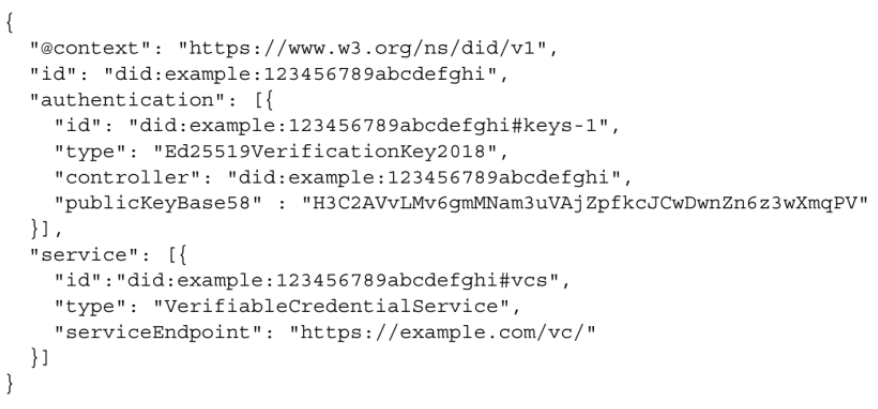
\includegraphics[width=0.6\textwidth]{5-Figures/DID.png}
    \caption{Exemplo de documento de DID com bloco de autenticação, chave pública, bloco de serviço e endpoint, como mencionado no ponto 4}
    \label{fig:did-example}
\end{figure}

\subsubsection{Tipos de DIDs}

Para encontrar a ferramenta certa para identificar utilizadores de forma descentralizada na rede Tor, é necessário compreender os diferentes tipos de DIDs que foram desenvolvidos desde a sua invenção.

Preukschat e Reed definem em 2021 as seguintes categorias de métodos DID desenvolvidas a partir de agosto de 2020 \cite{preukschat2021self}:

\begin{itemize}
    \item \textbf{(Ledger-based DIDs)} Categoria original de DID methods que envolvem uma \textit{blockchain} ou outra DLT, que envolve todas as operações numa ledger pública distribuída na rede com assinatura com chave privada do próprio;
    \item \textbf{(Ledger Middleware DIDs)} Melhoria dos Ledger-based DIDs, faz uso de uma camada intermédia entre o registo e o DID, de forma a que as transações possam ser agregadas para uma única entrada na tabela, otimizando o processo;
    \item \textbf{(Peer DIDs)} DIDs que não necessitam de uma camada pública de registo, operando exclusivamente através de redes peer-to-peer, possibilitando apenas a partilha do DID com apenas um peer ou grupo de peers, dando uso do protocolo de partilha da rede para a transmissão do identificador;
    \item \textbf{(Static DIDs)} Categoria de DIDs que permite criação e resolução, mas não permite alterações ou desativação, criados deterministicamente a partir de uma chave pública;
    \item \textbf{(Alternative DIDs)} Inovações de categorias de DIDs que não são contempladas nas categorias anteriores.
\end{itemize}

Alternativamente, Mazzocca et al. propõe uma categorização de DIDs focada no âmbito de partilha e na preservação da privacidade \cite{mazzocca2025survey}:

\begin{itemize}
    \item \textbf{(Anywise DIDs)} Identificadores públicos partilháveis com grupos ilimitados, mesmo se não forem confiáveis;
    \item \textbf{(Pairwise DIDs)} DID apenas conhecido pelo sujeito e por outra entidade, com foco principal na privacidade a partir de DIDs únicos para cada ligação sujeito-entidade, afastando possíveis ataques que usam a informação disponível para correlacionar dados com informação sensível;
    \item \textbf{(N-wise DIDs)} Desenhados de forma a que só possam ser conhecidos por N número de entidades, incluindo o sujeito. Caso N seja dois, é considerado um Pairwise DID.
\end{itemize}

A distinção entre estes tipos de DIDs - em particular os Pairwise DIDs e Peer DIDs - é crítica para a arquitetura proposta neste trabalho, permitindo determinar de que forma a partilha de credenciais previne correlation attacks na rede Tor.

\section{Fundamentos Algébricos}

\subsection{Curvas Elípticas}

Uma curva elíptica $E$ sobre um corpo $K$ é definida no plano pela equação geral de Weierstrass:

\begin{equation*}
    E : y^2 + a_1xy + a_3y = x^3 + a_2x^2 + a_4x + a_6
\end{equation*}

onde $a_1, a_2, a_3, a_4, a_6 \in K$ \cite{hankerson2004guide}.

Em aplicações criptográficas, trabalha-se maioritariamente sobre corpos finitos primos $\mathbb{F}_p$ com característica $p>3$. Nestas condições, através de uma mudança de variáveis, a equação de Weierstrass simplifica-se para a sua forma curta:

\begin{equation*}
    y^2 = x^3 + ax + b \pmod{p}
\end{equation*}

onde $a, b \in \mathbb{F}_p$. Para garantir que a curva é não-singular, isto é sem pontos duplos, o discriminante da curva deve satisfazer a condição $\Delta = 4a^3 + 27b^2 \pmod{p} \neq 0$. O conjunto de pontos $E(\mathbb{F}_p)$ é constituído por todos os pares $(x,y) \in \mathbb{F}_p \times \mathbb{F}_p$ que satisfazem a equação, acrescido de um elemento especial denominado ponto no infinito \cite{portnoi_ecc}.

O conjunto de pontos $E(\mathbb{F}_p)$ com a operação geométrica de adição de pontos forma um grupo abeliano finito, no qual o ponto no infinito $\mathcal{O}$ atua como o elemento neutro da adição ($P + \mathcal{O} = P$) \cite{hankerson2004guide}. A partir da adição de pontos, define-se a multiplicação escalar de um ponto $P \in E(\mathbb{F}_p)$ por um inteiro $k \in \mathbb{Z}_q^*$ como a adição sucessiva do ponto $P$ a si mesmo \cite{portnoi_ecc}:

\begin{equation*}
    kP = \underbrace{P + P + \ldots + P}_{k \text{ vezes}}
\end{equation*}

A segurança da criptografia baseada em curvas elípticas assenta na dificuldade em resolver o Problema do Logaritmo Discreto em Curvas Elípticas (\textit{Elliptic Curve Discrete Logarithm Problem} ou ECDLP). Dado um ponto gerador $P \in E(\mathbb{F}_p)$ e um ponto $Q = kP$, determina-se o valor do escalar secreto $k$, o que é computacionalmente inviável para corpos de dimensão adequada \cite{portnoi_ecc}.

\subsection{Emparelhamentos Bilineares}

O uso de emparelhamentos bilineares (\textit{bilinear pairings}) em criptografia ganhou relevância em 2000, quando Joux propôs uma variante tripartida do protocolo Diffie-Hellman baseada em curvas elípticas \cite{joux2000tripartite}. Esta abordagem fundamenta novos paradigmas criptográficos, desde Esquemas de Encriptação Baseados em Identidade (\textit{Identity-Based Encryption} - IBE) \cite{boneh2001ibe} até assinaturas curtas para canais com baixa largura de banda \cite{boneh2001short}.

Matematicamente, um emparelhamento bilinear é uma aplicação entre dois grupos de origem e um grupo de destino \cite{salin2023pairing}:

\begin{equation*}
    e : G_1 \times G_2 \longrightarrow G_T \, ,
\end{equation*}

onde $G_1$ e $G_2$ são dois grupos cíclicos de ordem prima $p$ definidos sobre curvas elípticas \cite{salin2023pairing} e $G_T$ é um grupo multiplicativo no corpo de extensão $\mathbb{F}_{p^k}$, tal que $|G_1| = |G_2| = |G_T| = p$.

A aplicação $e$ satisfaz três propriedades fundamentais \cite{salin2023pairing}:

\begin{enumerate}
    \item \textbf{(Bilinearity)} Para todos os pontos $P \in G_1$, $Q \in G_2$ e escalares $a, b \in \mathbb{Z}_p^*$:
    \begin{equation*}
        e(aP, bQ) = e(P, Q)^{ab}
    \end{equation*}
    \item \textbf{(Nondegeneracy)} Se $P$ for um gerador de $G_1$ e $Q$ for um gerador de $G_2$, então $e(P, Q) \neq 1 \in G_T$;
    \item \textbf{(Efficiently Computable)} Existe um algoritmo polinomial eficiente, como o algoritmo de Miller, para calcular $e(P, Q)$.
\end{enumerate}

\subsubsection{Tipos de Emparelhamentos Bilineares}

De acordo com a relação estrutural entre os grupos $G_1$ e $G_2$ e a existência de um homomorfismo que possa ser computado de forma eficiente $\psi : G_2 \rightarrow G_1$, os emparelhamentos classificam-se em quatro tipos \cite{salin2023pairing}:

\begin{itemize}
    \item \textbf{(Tipo 1 - Simétrico)} $G_1 = G_2$;
    \item \textbf{(Tipo 2)} $G_1 \neq G_2$ e $\exists \, \psi : G_2 \rightarrow G_1$, tal que $\psi$ é um homomorfismo computável de forma eficiente, e $\nexists \, H : \{0,1\}^* \rightarrow G_2$, sendo $H$ uma função de \textit{hash} eficiente com imagem em $G_2$ \cite{salin2023pairing};
    \item \textbf{(Tipo 3)} $G_1 \neq G_2$ e $\nexists \, \psi : G_2 \rightarrow G_1$, para a mesma definição de $\psi$;
    \item \textbf{(Tipo 4)} $G_1 \neq G_2$ e $\exists \, \psi : G_2 \rightarrow G_1$, para a mesma definição de $\psi$, e $\exists \, H : \{0,1\}^* \rightarrow G_2$, para a mesma definição de $H$.
\end{itemize}

\subsubsection{Garantias de Segurança e a Curva BLS12-381}

A segurança dos esquemas baseados em emparelhamentos simétricos assenta no Problema de Diffie-Hellman Bilinear (BDH) \cite{boneh2001ibe}. Dado um gerador de parâmetros que produz $\langle G_1, G_T, e, P \rangle$, o problema consiste em computar $e(P,P)^{abc} \in G_T$ a partir da instância $(P, aP, bP, cP)$ para $a,b,c \in \mathbb{Z}_p$. A hipótese BDH assume que nenhum algoritmo de tempo polinomial tem vantagem não-negligenciável $Adv(q)$ na resolução deste problema \cite{boneh2001ibe}.

Entre os tipos apresentados, os emparelhamentos do (Tipo 3) revelam-se especialmente relevantes para este trabalho. Destaca-se a curva de Barreto-Lynn-Scott (BLS12-381), definida pela equação $y^2 = x^3 + 4$ sobre o corpo finito $\mathbb{F}_q$, com um primo $q$ de 381 bits \cite{salin2023pairing, electriccoin_bls12381}. A utilização desta curva garante um nível de segurança de 128 bits com um desempenho otimizado e dimensões reduzidas de elementos em $G_1$.

A garantia de segurança do uso da curva elíptica BLS12-381 baseia-se numa variante do problema BDH adaptada a grupos assimétricos ($G_1 \neq G_2$), denominada Problema da Inversão de Diffie-Hellman Bilinear de Decisão de ordem $q$ ($q$-DBDHI). Dado um gerador $P \in G_1$, um gerador $P' \in G_2$ e o tuplo de elementos:

\begin{equation*}
    (P, yP, y^2P, \ldots, y^qP, P', R)
\end{equation*}

para $y \in \mathbb{Z}_p$ e $R \in G_T$, o problema consiste em determinar se $R = e(P,P')^{1/y}$ ou se $R$ é um elemento aleatório de $G_T$ \cite{salin2023pairing}.

A adoção de emparelhamentos assimétricos do (Tipo 3) sobre a curva BLS12-381 maximiza a eficiência computacional e a segurança, sendo ideal para mitigar restrições de largura de banda na transmissão de mensagens pela rede.

\section{Primitivas Criptográficas}

\subsection{Pedersen Commitment}

Os esquemas de compromisso (\textit{commitment schemes}) constituem uma primitiva criptográfica fundamental que permite a uma parte comprometer-se com um valor secreto sem o revelar, podendo ser usado de forma a provar relações entre o mesmo e outros valores de compromisso do mesmo utilizador, sem providenciar informação adicional que possa revelar o valor secreto \cite{yu2020simple}.

Torben Pedersen propôs um esquema de compromisso baseado na dureza do Problema do Logaritmo Discreto. Para um grupo cíclico $G_q$ de ordem prima $q$, gerado sobre um subgrupo de $\mathbb{Z}_p^*$, onde $p$ e $q$ são primos de grande dimensão tais que $p-1$ é divisível por $q$. Sejam $g$ e $h$ dois geradores de $G_q$ escolhidos de forma a que o valor $x = \log_g h$ seja desconhecido para todas as partes \cite{reaction_la_pedersen}. Para se comprometer com um valor secreto $m \in \mathbb{Z}_q$, a entidade emissora seleciona um valor aleatório $r \in \mathbb{Z}_q$ (\textit{blinding factor}) e calcula o compromisso $c \in G_q$ \cite{reaction_la_pedersen}:

\begin{equation*}
    c = \mathrm{Com}(m, r) = g^m h^r \pmod{p}
\end{equation*}

\subsubsection{Fases do Pedersen Commitment}

O protocolo do compromisso de Pedersen entre um emissor $C$, que detém o segredo $m$, e um verificador $R$, decorre em duas fases \cite{metere2017automated}:

\begin{itemize}
    \item \textbf{Fase de Compromisso:}
    \begin{itemize}
        \item Os parâmetros públicos do grupo $(G_q, q, g, h)$ são definidos;
        \item $C$ escolhe uniformemente $r \xleftarrow{R} \mathbb{Z}_q$, calcula $c = g^m h^r \pmod{p}$ e envia-o para $R$.
    \end{itemize}
    \item \textbf{Fase de Verificação:}
    \begin{itemize}
        \item $C$ revela o par $(m, r)$ a $R$;
        \item $R$ verifica se $c = g^m h^r \pmod{p}$. Caso a igualdade se verifique, aceita o compromisso, caso contrário rejeita-o.
    \end{itemize}
\end{itemize}

\subsubsection{Propriedades de Segurança}

O compromisso de Pedersen garante três propriedades fundamentais \cite{pedersen1991noninteractive}:

\begin{itemize}
    \item \textbf{(Perfect Hiding)} Para quaisquer mensagens $m, m' \in \mathbb{Z}_q$, as distribuições dos compromissos $Com(m,r)$ e $Com(m',r')$ são estatisticamente indistinguíveis quando $r,r' \xleftarrow{R} \mathbb{Z}_q$. Portanto, o compromisso $c$ não revela qualquer informação sobre $m$, mesmo perante um adversário com poder computacional ilimitado;
    \item \textbf{(Computationally Binding)} Assumindo a intratabilidade do logaritmo discreto em $G_q$, a probabilidade de um adversário de tempo polinomial encontrar um segundo par $(m',r')$ tal que $m' \neq m$ e $Com(m,r) = Com(m',r')$ é negligenciável;
    \item \textbf{(Homomorfismo Aditivo)} Para quaisquer mensagens $m_1, m_2 \in \mathbb{Z}_q$ e \textit{blindness factors} $r_1, r_2 \in \mathbb{Z}_q$, a multiplicação dos compromissos resulta no compromisso da soma das mensagens e dos fatores de aleatoriedade:
    \begin{align*}
        Com(m_1, r_1) \cdot Com(m_2, r_2) &= (g^{m_1}h^{r_1}) \cdot (g^{m_2}h^{r_2}) \\
        &= g^{m_1+m_2}h^{r_1+r_2} = Com(m_1+m_2, r_1+r_2)
    \end{align*}
\end{itemize}

Estas propriedades são determinantes para a arquitetura de mitigação de \textit{Sybil attacks} na rede Tor, permitindo que o operador de um nó oculte a sua identidade real ou atributos ao solicitar credenciais às \textit{Directory Authorities}, provando relações algébricas sobre os seus dados sem os expor.

\subsection{Encriptação de ElGamal}

Taher ElGamal \cite{elgamal1985public} introduziu um novo esquema de encriptação de chave pública probabilístico e com propriedades homomórficas \cite{brandt2005efficient}, cujo esquema opera sobre um grupo cíclico $G_q$ de ordem prima $q$ com gerador $g$, sendo composto por três algoritmos fundamentais \cite{crites2025syra}:

\begin{itemize}
    \item \textbf{(Geração de Chaves)} Dado um parâmetro de segurança $1^\lambda$, o algoritmo seleciona uma chave secreta $sk = x \xleftarrow{R} \mathbb{Z}_q^*$ de forma uniformemente aleatória e computa o componente correspondente da chave pública $P = g^x \in G_q$. A chave pública é definida como $pk = (G_q, q, g, P)$ e a chave privada como $sk = x$;
    \item \textbf{(Encriptação)} Para encriptar uma mensagem $M \in G_q$, o emissor escolhe um valor aleatório efémero $r \xleftarrow{R} \mathbb{Z}_q^*$ e calcula o texto cifrado $C = (C_1, C_2)$:
    \begin{equation*}
        C_1 = g^r \pmod{p}, \quad C_2 = P^r \cdot M \pmod{p}
    \end{equation*}
    \item \textbf{(Desencriptação)} Dado um texto cifrado $C = (C_1, C_2)$, o recetor utiliza a chave privada $sk = x$ para recuperar a mensagem original:
    \begin{equation*}
        M = \frac{C_2}{(C_1)^x} = \frac{P^r \cdot M}{(g^r)^x} = \frac{(g^x)^r \cdot M}{(g^r)^x} = M
    \end{equation*}
\end{itemize}

A segurança semântica do esquema de ElGamal contra ataques de texto claro escolhido (IND-CPA) baseia-se diretamente na intratabilidade do Problema de Diffie-Hellman de Decisão (DDH) no grupo $G_q$ \cite{crites2025syra}.

\subsubsection{Propriedades do Esquema}

O esquema de ElGamal possui duas propriedades estruturais determinantes para a construção de protocolos criptográficos avançados \cite{brandt2005efficient}:

\begin{itemize}
    \item \textbf{(Homomorfismo Multiplicativo)} Dados dois textos cifrados $C^{(1)} = (g^{r_1}, P^{r_1}M_1)$ e $C^{(2)} = (g^{r_2}, P^{r_2}M_2)$ resultantes da encriptação das mensagens $M_1$ e $M_2$, o produto entre os componentes dos criptogramas produz um texto cifrado válido para a mensagem $M_1 \cdot M_2$:
    \begin{equation*}
        C^{(1)} \cdot C^{(2)} = (g^{r_1+r_2}, P^{r_1+r_2}(M_1 \cdot M_2)) = Enc(M_1 \cdot M_2, r_1+r_2)
    \end{equation*}
    O esquema padrão não é aditivamente homomórfico para os \textit{plaintexts}, a menos que a mensagem seja codificada no expoente ($g^M$), variante conhecida como \textit{Additive ElGamal} \cite{ge2024hybrid};
    \item \textbf{(Encriptação Probabilística)} A utilização do fator efémero aleatório $r$ assegura que duas encriptações da mesma mensagem $M$ produzem textos cifrados completamente distintos \cite{elgamal1985public}.
\end{itemize}

\subsubsection{ElGamal sobre Curvas Elípticas}

A adaptação do esquema de ElGamal para grupos de curvas elípticas surge da necessidade de aumentar a velocidade do processo de encriptação e desencriptação dos esquemas de criptografia de chave pública \cite{ieee5620105_ecelgamal}.

A transição para curvas elípticas reduz a dimensão das chaves e o custo computacional. Além das melhorias de eficiência, permite a sua integração direta com esquemas de criptografia limiar, cujo funcionamento descentralizado e mecanismos de partilha de segredos serão aprofundados na secção dedicada a esse tema \cite{ieee5620105_ecelgamal}.

\subsection{Verifiable Random Functions}

Uma \textit{Verifiable Random Function} (VRF) é uma função criptográfica cujo resultado é pseudoaleatório e acompanhado de uma prova publicamente verificável \cite{david2024musen}. Utilizando uma chave secreta ($SK$), o detentor gera um valor de saída e uma prova associada, de modo a que qualquer entidade em posse da chave pública ($PK$) correspondente pode verificar a validade do cálculo sem ter acesso ao segredo.

As VRFs constituem pilares criptográficos em sistemas com entidades responsáveis pela execução de tarefas, como \textit{blockchains} baseadas em \textit{Proof-of-Stake} para seleção de líderes e sorteios \cite{david2024musen}. Micali e Rivest também usaram VRFs para construir esquemas de micropagamentos para sistemas de lotaria não interativos, reduzindo a complexidade de verificação de saldo \cite{micali2002micropayments}.

\subsubsection{Definição Formal}

A noção formal de VRF foi introduzida por Micali, Rabin e Vadhan como uma tupla de algoritmos em tempo polinomial $(G, F, V)$ \cite{micali1999verifiable}:

\begin{itemize}
    \item \textbf{(Gerador Probabilístico - G)} Recebe o parâmetro de segurança $1^k$ e produz o par de chaves públicas e secretas $(PK, SK)$;
    \item \textbf{(Avaliador Determinístico - F)} Definido por $F = (F_1, F_2)$, recebe a chave secreta $SK$ e uma entrada $x$, produzindo o resultado $y = F_1(SK, x)$ e a prova correspondente $\pi = F_2(SK, x)$;
    \item \textbf{(Verificador Probabilístico - V)} Recebe o contexto $(PK, x, y, \pi)$ e retorna um valor \textit{boolean} $\{0, 1\}$.
\end{itemize}

\subsubsection{VRF de Dodis-Yampolskiy}

Yevgeniy Dodis e Aleksandr Yampolskiy apresentam uma construção eficiente e simples de VRF baseada em grupos bilineares de ordem prima $p$, composta por três algoritmos \cite{dodis2005verifiable}:

\begin{itemize}
    \item $Gen(1^k)$: Seleciona um valor aleatório $s \xleftarrow{R} \mathbb{Z}_p^*$ e define a chave secreta $SK = s$ e a chave pública $PK = g^s$;
    \item $Prove_{SK}(x)$: Calcula o resultado da VRF $y$ e a prova $\pi$:
    \begin{equation*}
        y = F_{SK}(x) = e(g,g)^{\frac{1}{x+SK}}, \quad \pi_{SK}(x) = g^{\frac{1}{x+SK}}
    \end{equation*}
    \item $Ver_{PK}(x,y,\pi)$: Valida o resultado verificando se as seguintes igualdades bilineares são satisfeitas:
    \begin{equation*}
        e(g^x \cdot PK, \pi) = e(g,g) \quad \text{e} \quad y = e(g, \pi) \, ,
    \end{equation*}
    e retorna 1 se ambas forem verdadeiras e 0 caso contrário.
\end{itemize}

A segurança das VRF de Dodis e Yampolskiy, ou DY-VRF, fundamenta-se na dureza do problema de Inversão de Diffie-Hellman Bilinear de Decisão de ordem $q$ ($q$-DBHI). Este problema estabelece que, dado o tuplo de elementos $(g, g^x, g^{x^2}, \ldots, g^{x^q})$, é computacionalmente difícil distinguir $e(g,g)^{1/x}$ de um valor aleatório de $G_T$ \cite{crites2025syra}. Esta construção garante o anonimato do utilizador, a verificabilidade por terceiros \cite{crites2025syra} e assegura um tamanho constante para as chaves e provas de verificação, independentemente da dimensão dos dados de entrada \cite{dodis2005verifiable}.

\subsection{Zero-Knowledge Proofs}

As \textit{Zero-Knowledge Proofs} (ZKPs) constituem um protocolo criptográfico que permite a uma entidade, o provador ($P$), demonstrar a uma segunda entidade, o verificador ($V$), a veracidade de uma afirmação sem revelar qualquer informação adicional para além da própria validade da mesma \cite{mulder2023trends}.

\subsubsection{Tipos de Zero-Knowledge Proofs}

As \textit{Zero-Knowledge Proofs} dividem-se em dois modelos principais, que diferem pela necessidade de interação direta entre as partes, e pela capacidade de transferência da prova a terceiros.

\textbf{ZKPs Interativas.} É possível definir um sistema de prova interativo a partir de um par de algoritmos $(P, V)$, onde $P$ atua como a entidade que efetua a prova e $V$ como a entidade que verifica. Como protocolo de linguagem da prova, define-se $L \subseteq \{0,1\}^*$ e um valor de entrada partilhado entre $P$ e $V$, $x \in L$. $P$ e $V$ trocam uma sequência de mensagens $(p_1, v_1, p_2, v_2, \ldots, p_n, v_n)$, que faz uso de cada par $(p_i, v_i)$ partilhado em tempo polinomial $|x|$ para realizar a prova $(P,V)(x) \in \{Accept, Reject\}$, cuja resposta reflete a decisão de $V$ relativa à alegação de $P$ sobre $x \in L$ \cite{kurmi2015survey}.

Como explicação de uma ZKP interativa, pode-se simplificar um caso de iterações real, em que Alice quer provar a Bob, que é daltónico, que duas bolas têm cores diferentes. Para isto, sem o conhecimento de Alice, Bob muda ou não a ordem das bolas, e segue da resposta de Alice sobre se as bolas mudaram de ordem ou não. Após várias iterações, é possível para Bob decidir se a alegação de Alice, isto é que as duas bolas têm cores diferentes, é verdadeira ou falsa, sem recurso a mais nenhuma informação extra \cite{mulder2023trends}. Contudo, as provas interativas não são transferíveis a terceiros, ou seja uma gravação de uma interação entre $P$ e $V$ não serve como prova para uma terceira parte, dado que $V$ poderia ter conluiado com $P$ ou gerado a gravação autonomamente através de um simulador.

\textbf{ZKPs Não-Interativas.} Para superar a limitação da interatividade e permitir a verificação por múltiplas entidades, Blum, Feldman e Micali \cite{blum2019non} introduziram as \textit{Non-Interactive Zero Knowledge Proofs} (NIZKPs). Neste modelo, $P$ e $V$ partilham uma \textit{string} aleatória denominada de \textit{common reference string} (CRS), e é usado como segredo para o protocolo de prova para a construção de desafios verificáveis.

Ao contrário do modelo interativo, as NIZKPs são publicamente verificáveis e transferíveis, de modo a que qualquer entidade na posse da CRS e da prova possa comprovar de forma autónoma a veracidade de $x \in L$, sem a necessidade de estabelecer um canal de comunicação bidirecional com o provador nem arriscar a fuga de dados secretos \cite{mulder2023trends}.

\subsubsection{Propriedades Fundamentais das ZKPs}

Para que um protocolo de prova seja classificado como uma ZKP válida, deve satisfazer três propriedades fundamentais \cite{mulder2023trends}:

\begin{itemize}
    \item \textbf{(Completeness)} Se a afirmação $x \in L$ for verdadeira e se ambos $P$ e $V$ seguirem honestamente o protocolo, então $V$ pode verificar que a alegação é verdadeira;
    \item \textbf{(Soundness)} Se a afirmação for falsa, ($x \notin L$), nenhum provador desonesto, mesmo com capacidade computacional ilimitada, conseguirá convencer um verificador honesto a aceitar a prova \cite{kurmi2015survey}. Por outras palavras, se a afirmação for falsa, então $V$ poderia verificar que a alegação é falsa;
    \item \textbf{(Zero-Knowledge)} Se $x \in L$, o verificador não obtém qualquer informação além do facto de que a afirmação é verdadeira.
\end{itemize}

\subsubsection{Prova de Schnorr e DLEQs}

Schnorr propôs um esquema de identificação interativo eficiente, baseado na intratabilidade do Problema do Logaritmo Discreto \cite{schnorr1989efficient, schnorr1991efficient}. O protocolo de Schnorr permite que uma entidade $P$ demonstre a uma entidade verificadora $V$, de forma \textit{Zero-Knowledge}, o conhecimento do logaritmo discreto $x$ associado a uma chave pública $y = g^x$.

Seja $G = \langle g \rangle$ um grupo cíclico de ordem prima $q$ com gerador $g$. O protocolo interativo decorre em três passos \cite{paillier2005discretelog}:

\begin{enumerate}
    \item \textbf{(Compromisso)} $P$ seleciona um valor efémero aleatório $k \xleftarrow{R} \mathbb{Z}_q^*$, calcula o compromisso $r = g^k \in G$ e envia $r$ para $V$;
    \item \textbf{(Desafio)} $V$ escolhe um valor aleatório $c \xleftarrow{R} \mathbb{Z}_q$ e envia-o para $P$;
    \item \textbf{(Resposta)} $P$ calcula a resposta $s = k + cx \pmod{q}$ e envia-a para $V$.
\end{enumerate}

O verificador $V$ aceita a prova se e só se a seguinte igualdade se verificar em $G$:

\begin{equation*}
    g^s = r \cdot y^c
\end{equation*}

Substituindo $s$ e $y$, observa-se que $g^s = g^{k+cx} = g^k \cdot (g^x)^c = r \cdot y^c$, concluindo que $P$ conhece o segredo $x$ sem o expor.

\subsubsection{Heurística de Fiat-Shamir}

Para converter o protocolo interativo de Schnorr numa NIZKP, aplica-se a Heurística de Fiat-Shamir \cite{fiatshamir1986how}. Esta transformação substitui a presença de um verificador interativo na fase de desafio pelo cálculo determinístico do desafio através de uma função de \textit{hash} criptográfica publicamente acessível $H : \{0,1\}^* \rightarrow \mathbb{Z}_q$.

Nesta variante não-interativa:

\begin{itemize}
    \item A entidade que prova, $P$, gera $k \xleftarrow{R} \mathbb{Z}_q^*$, calcula $r = g^k$ e computa autonomamente o desafio $c$ sobre os elementos públicos do protocolo, $c = H(g \, || \, y \, || \, r)$;
    \item $P$ calcula $s = k + cx \pmod{q}$ e publica o par de prova $\pi = (c, s)$ ou $\pi = (r, s)$.
\end{itemize}

Para verificar a prova $\pi = (c, s)$, qualquer entidade externa $V$ calcula $r' = g^s \cdot y^{-c}$ e valida se $H(g \, || \, y \, || \, r') = c$ \cite{fiatshamir1986how}.

A segurança da transformação de Fiat-Shamir é provada no Modelo do Oráculo Aleatório (\textit{Random Oracle Model} - ROM), garantindo que a prova não-interativa resultante é publicamente verificável, transferível e computacionalmente equivalente ao protocolo interativo original \cite{fiatshamir1986how}.

\subsubsection{Prova de Igualdade de Logaritmos Discretos}

Uma \textit{Discrete Logarithm Equality Proof} ou DLEQ é uma NIZKP de igualdade de logaritmos discretos, que permite demonstrar que dois pares de elementos de um grupo têm o mesmo logaritmo discreto, sem o revelar \cite{rfc9497}. Esta prova foi desenvolvida por Chaum e Pedersen \cite{chaumpedersen1992wallet}, sendo mais tarde provada ZK por Jarecki et al. \cite{jarecki2014roundoptimal} e transformada em não interativa pela Heurística de Fiat-Shamir \cite{fiatshamir1986how}.

A prova de Schnorr não é suficiente em casos onde queremos provar que o mesmo segredo está por trás de duas chaves públicas diferentes, potencialmente em grupos diferentes. É nesta medida que o DLEQ é criado. Dados dois pares $(g, y = g^x)$ e $(h, z = h^x)$, a prova demonstra conhecimento de um único $x$ que satisfaz ambas as relações em simultâneo. O esquema está estruturado como uma prova de Schnorr, excetuando dois compromissos ao invés de apenas um, $r_1 = g^k$ e $r_2 = h^k$, usando o mesmo $k$ aleatório nos dois e uma resposta partilhada. O desafio calculado é transformado pela Heurística de Fiat-Shamir, usando apenas um para ambos os compromissos:

\begin{equation*}
    c = H(g \, || \, y \, || \, h \, || \, z \, || \, r_1 \, || \, r_2)
\end{equation*}

É o uso de um só desafio para ambos os compromissos que garante que o $x$ usado é o mesmo para ambas as relações. Por fim, a DLEQ é verificada por duas igualdades, com o mesmo $s$ e $c$:

\begin{equation*}
    g^s = r_1 \cdot y^c \quad \text{e} \quad h^s = r_2 \cdot z^c
\end{equation*}

A DLEQ é usada no Dittor para ligar o pseudónimo à credencial emitida pelas CAs, com uma variante bilinear aplicável a sistemas com emparelhamentos bilineares.

\section{Threshold Cryptography}

A criptografia limiar (\textit{Threshold Cryptography}) surge da necessidade de descentralizar a confiança em sistemas computacionais, distribuindo capacidades criptográficas (como desencriptação ou geração de assinaturas) por um conjunto de $n$ entidades, de forma a eliminar pontos únicos de falha.

\subsection{Shamir Secret Sharing}

A técnica de partilha secreta proposta por Shamir permite dividir um segredo $s$ em $n$ partes, podendo reconstruí-lo facilmente a partir de qualquer subconjunto de pelo menos $t$ partes. O esquema garante segurança perfeita ao nível da teoria da informação (\textit{information-theoretic security}): caso se obtenha conhecimento de $t-1$ (ou menos) partes, não é possível obter nenhuma informação sobre o segredo $s$ \cite{shamir1979how}.

A infraestrutura tradicional do esquema envolve uma entidade central responsável - o \textit{Dealer} - por calcular cada parte e distribuir os resultados, de forma segura, para as outras $n$ entidades. A reconstrução do segredo é efetuada através do envio de cada parte de volta para a entidade central, podendo então combinar todas as partes para recuperar $s$, necessitando apenas de pelo menos $t$ partes para o fazer \cite{bogdanov_shamir_notes}.

O esquema de partilha de segredos limiar $(t,n)$ é definido sobre o corpo finito $\mathbb{Z}_p$, com $p > n$ e $p > s$, por dois algoritmos \cite{crites2025syra}:

\begin{itemize}
    \item \textbf{$Share_{t,n}(s)$}: Dado o segredo $s \in \mathbb{Z}_p$, o algoritmo escolhe aleatoriamente $t-1$ coeficientes $a_1, a_2, \ldots, a_{t-1} \xleftarrow{R} \mathbb{Z}_p$ e constrói um polinómio de grau $t-1$:
    \begin{equation*}
        P(x) = s + a_1x + a_2x^2 + \ldots + a_{t-1}x^{t-1} \pmod{p}
    \end{equation*}
    O segredo encontra-se codificado no termo independente, $P(0) = s$. O algoritmo gera $n$ partes $s_i = (x_i, y_i)$, onde $y_i = P(x_i)$ e cada $x_i \in \mathbb{Z}_p \setminus \{0\}$ é um identificador único e não-nulo atribuído à $i$-ésima entidade;
    \item \textbf{$Reconstruct_{t,n}(\{s_i\}_{i \in I})$}: Dado um subconjunto $I \subseteq \{1, \ldots, n\}$ de partes de dimensão $|I| = t$, o segredo $s = P(0)$ é reconstruído deterministicamente através da interpolação de Lagrange sobre $x = 0$:
    \begin{equation*}
        s = P(0) = \sum_{i \in I} y_i \cdot l_i(0) \pmod{p}
    \end{equation*}
    onde $l_i(0)$ representa o $i$-ésimo coeficiente/polinómio de base de Lagrange avaliado em 0:
    \begin{equation*}
        l_i(0) = \prod_{j \in I, j \neq i} \frac{x_j}{x_j - x_i} \pmod{p}
    \end{equation*}
\end{itemize}

É importante sublinhar que os identificadores $x_i$ de cada participante devem satisfazer $x_i \neq 0$, dado que a posição $x=0$ é estritamente reservada para armazenar e avaliar o segredo $s$ \cite{bogdanov_shamir_notes}.

\subsection{Distributed Key Generation}

A Geração Distribuída de Chaves (\textit{Distributed Key Generation} - DKG) resolve a vulnerabilidade da centralização em esquemas de partilha de segredos tradicionais, nos quais uma entidade confiável (\textit{Trusted Dealer}) é responsável por gerar e distribuir o par de chaves.

Dada a natureza de partilha de atributos secretos aprofundada por Shamir, a geração distribuída de chaves torna-se um componente principal de sistemas de criptografia limiar, permitindo que um conjunto de $n$ servidores criem em conjunto um par de chaves pública e privada a partir de uma distribuição pré-acordada do sistema, sem necessidade de computar, reconstruir ou guardar uma chave secreta numa localização única, ou confiar numa entidade central \cite{gennaro2007secure}. As propriedades de segurança mantêm-se ao garantir que um atacante não obtém informações sobre a chave secreta desde que não comprometa um número de entidades superior ao limiar \cite{gennaro2007secure}.

Formalmente, o DKG permite que um conjunto de $n$ servidores possa gerir cooperativamente um par de chaves pública e privada $(y,x)$, no qual a chave pública $y = g^x$ é conhecida por todos os participantes, mas a chave secreta $x \in \mathbb{Z}_q^*$ nunca é reconstruída ou armazenada numa única localização. Cada participante $i$ obtém apenas uma fração secreta $x_i$, garantindo a segurança do sistema enquanto o número de entidades comprometidas for inferior ao limiar $t$ \cite{gennaro2007secure}.

\subsection{Pedersen's DKG e Verifiable Secret Sharing}

Torben Pedersen propõe o primeiro esquema de geração distribuída de chaves baseado em partilha de segredos verificáveis \cite{gennaro2007secure} como resposta à necessidade de um meio de partilha de segredos sem uma entidade central responsável pela partilha dos mesmos \cite{pedersen1991threshold}.

Um esquema de geração distribuída de chaves com possibilidade dos seus membros verificarem, sem necessidade de interações adicionais, que a sua parte das chaves é matematicamente consistente com as dos restantes membros é classificado como um esquema de partilha de segredos verificáveis. Até então, foram apresentados esquemas deste género interativos, limitando os membros do sistema a interagirem entre si para verificar a validade da sua parte, o que motiva Pedersen a encontrar uma solução não interativa \cite{reaction_la_pedersen}. Para isto, implementa um esquema de partilha de segredos verificáveis que faz uso de compromissos de Pedersen com partilha de segredos de Shamir, adicionando os compromissos aos coeficientes do polinómio

\begin{equation*}
    f(x) = s + a_1x + \ldots + a_{t-1}x^{t-1}
\end{equation*}

\cite{reaction_la_pedersen}.

Para eliminar a necessidade da entidade central distribuidora, o protocolo de DKG de Pedersen executa $n$ instâncias paralelas do seu esquema de partilha de segredos verificáveis em paralelo, decorrendo da seguinte forma \cite{pedersen1991threshold}:

\begin{itemize}
    \item \textbf{(Geração de Polinómios Locais)} Cada participante $i \in \{1, \ldots, n\}$ escolhe aleatoriamente um segredo local $z_i \xleftarrow{R} \mathbb{Z}_q^*$ e dois polinómios aleatórios de grau $t-1$:
    \begin{align*}
        f_i(x) &= a_{i,0} + a_{i,1}x + \ldots + a_{i,t-1}x^{t-1} \pmod{q}, \\
        g_i(x) &= b_{i,0} + b_{i,1}x + \ldots + b_{i,t-1}x^{t-1} \pmod{q};
    \end{align*}
    \item \textbf{(Distribuição e Compromisso)} Cada participante $i$ envia o par de partes $s_{ij} = f_i(j) \pmod{q}$ e $t_{ij} = g_i(j) \pmod{q}$ ao participante $j$ e publica os compromissos de Pedersen, que cobrem os coeficientes do polinómio local de cada participante $i$:
    \begin{equation*}
        C_{i,k} = g^{a_{i,k}} h^{b_{i,k}} \pmod{p} \quad \text{para } k = 0, \ldots, t-1;
    \end{equation*}
    \item \textbf{(Verificação Local)} Cada participante $j$ aceita as partes recebidas de $i$ se e só se a seguinte igualdade for satisfeita:
    \begin{equation*}
        g^{s_{ij}} h^{t_{ij}} = \prod_{k=0}^{t-1} (C_{i,k})^{j^k} \pmod{p};
    \end{equation*}
    \item \textbf{(Agregação de Chaves)} Se nenhuma parte for desqualificada, a chave privada global é $x = \sum_{i=1}^{n} z_i \pmod{q}$, e a fração da chave secreta retida por cada nó $j$ é $x_j = \sum_{i=1}^{n} f_i(j) \pmod{q}$. A chave pública global é obtida multiplicando os componentes públicos $A_{i,0} = g^{z_i}$:
    \begin{equation*}
        y = \prod_{i=1}^{n} g^{z_i} = g^x \pmod{p}.
    \end{equation*}
\end{itemize}

\subsection{Vulnerabilidade e o Ataque de Gennaro et al.}

O esquema de geração distribuída de chaves de Pedersen foi modificado ao longo dos anos, tornando-se um pilar importante neste género de esquemas criptográficos \cite{gennaro2007secure}. No entanto, Gennaro et al. mostram que o esquema de Pedersen não garante que a chave pública resultante seja distribuída de forma uniformemente aleatória, formalizando uma ameaça válida \cite{gennaro2007secure}.

Um adversário que controle um conjunto de participantes corruptos pode aguardar até que todos os nós honestos publiquem os seus compromissos $C_{i,k}$. Conhecendo os valores $g^{z_i}$ dos nós honestos, o adversário pode decidir estrategicamente quais os nós identidades desqualificar (por exemplo, simulando falhas ou recusando publicar justificações), forçando a reconstrução ou remoção de certas contribuições $z_i$. Ao escolher quais os segredos $z_i$ que entram no somatório final, o adversário consegue enviesar os bits menos significativos da chave pública $y = g^{\sum z_i}$ \cite{gennaro2007secure}.

Para mitigar este ataque, Gennaro et al. propuseram um novo protocolo de geração distribuída de chaves com distribuição garantidamente uniforme, cujo custo computacional considera-se bastante elevado, o que leva à procura de novas soluções \cite{das2023scalable_dkg, kate2026scalable}.

\subsection{Partial Blind Signatures}

As assinaturas cegas (\textit{Blind Signatures}) foram introduzidas por Chaum \cite{chaum1982blind} e atualmente são primitivas essenciais no mundo da criptografia, permitindo que duas entidades, uma entidade assinante com posse de uma chave secreta e outra com uma mensagem, criem em conjunto uma assinatura \cite{kastner2022abeokamoto}. Este tipo de assinaturas satisfazem duas características principais \cite{ieee4533332_blindsig}:

\begin{itemize}
    \item \textbf{(Blindness)} Uma assinatura cega permite que uma entidade assine uma mensagem $m$ de um utilizador sem aprender nenhuma informação sobre a mesma, nem mesmo usar nenhuma informação que divulgue quando é que $m$ foi assinada, contudo permitindo que ambas as partes verifiquem a identidade do assinante;
    \item \textbf{(One-More Unforgeability)} É impossível para um utilizador obter $k+1$ assinaturas válidas após interagir apenas $k$ vezes com a entidade que assina.
\end{itemize}

As assinaturas cegas são essenciais no mundo do comércio eletrónico, dado permitirem que uma entidade autorize documentos digitais que se deslocam frequentemente entre redes \cite{pointcheval2000security}.

O conceito de assinaturas cegas parciais foi introduzido para mitigar o problema de escalabilidade no armazenamento de associações entre assinaturas e objetos assinados que surgiu nas bases de dados dos bancos, dado ser necessário manter todas as assinaturas guardadas para prevenir o gasto múltiplo de um só recurso \cite{ieee4533332_blindsig}. Este conceito foi introduzido por Abe e Fujisaki \cite{abefujisaki1996date} como uma extensão de uma assinatura cega, permitindo a um assinante incluir, em conjunto com o requerente da assinatura, informação adicional visível na mesma \cite{kastner2022abeokamoto}. Esta noção foi formalizada e provada segura por Abe e Okamoto \cite{abeokamoto2000partial}.

As assinaturas cegas parciais permitem que o utilizador e o assinante cheguem a um acordo e incluam uma \textit{string} de informação pública e não cega $info$ no processo de assinatura \cite{kastner2022abeokamoto}:

\begin{enumerate}
    \item \textbf{(Acordo sobre Metadados)} O utilizador e o assinante concordam abertamente sobre o conteúdo de $info$;
    \item \textbf{(Cegueira Selecionável)} O utilizador aplica um \textit{blinding factor} à sua mensagem privada $m$, mantendo-a oculta, mas envia $info$ em \textit{plaintext} para o assinante;
    \item \textbf{(Geração e Verificação)} O assinante gera a assinatura parcial ponderando a chave secreta $sk$, a mensagem ofuscada e os metadados $info$. O resultado é um par $(m, \sigma)$ cuja validade é verificável publicamente em relação à chave pública do assinante $pk$ e aos metadados agregados:
    \begin{equation*}
        Verify(pk, m, info, \sigma) \in \{0, 1\}
    \end{equation*}
\end{enumerate}

Desta forma, preserva-se o anonimato do utilizador relativamente ao conteúdo específico de $m$, permitindo que o sistema aplique regras públicas à assinatura através de $info$.

\section{Babel}

O Babel \cite{fouto2022babel} é uma \textit{framework} em Java que providencia um ambiente de programação para implementar protocolos distribuídos e sistemas, simplificando mecanismos habituais de forma a estender o seu uso para ser mais abrangente. Este mecanismo funciona de forma a que um processo possa executar um número arbitrário de protocolos diferentes, permitindo que o desenvolvedor do projeto possa focar-se na sua lógica principal, sem necessidade de resolução de problemas típicos de sistemas distribuídos \cite{fouto2022babel}.

O modelo do Babel é orientado a eventos, de forma a abstrair detalhes de baixo nível como concorrência, entrega de mensagens e gestão de redes \cite{pereira2025decentralized}. A arquitetura da \textit{framework} consiste em três componentes: protocolos implementados como máquinas de estado com filas de eventos para execução independente e concorrente, um núcleo responsável por coordenar interações entre processos e dentro dos mesmos, e canais de comunicação com abstrações flexíveis de vários mecanismos de comunicação \cite{pereira2025decentralized}.

A implementação do Babel permite que um programador possa implementar a sua solução com tolerância a falhas e aspetos de dependência de sistemas distribuídos sem necessidade de lidar com aspetos de redes de baixo nível, tal como problemas de concorrência que surgem na sua implementação \cite{fouto2022babel}.

\section{SyRA - Sybil-Resilient Anonymous Signatures with Applications to Decentralized Identity}

O esquema \textit{SyRA} (\textit{Sybil-Resilient Anonymous Signatures}) é uma primitiva criptográfica desenhada para reconciliar a verificação de identidade no mundo real com a preservação do anonimato e a prevenção de ataques \textit{Sybil} em sistemas descentralizados \cite{crites2025syra}. Estas assinaturas são usadas de forma a complementar uma credencial verificável da identidade real do sujeito, que pode ser obtida a partir de qualquer identificador legal (como o Cartão de Cidadão português), biométrico (como a impressão digital) ou a partir de qualquer método legal capaz de identificação como o OpenID Connect \cite{openid_connect}, por exemplo, garantindo o princípio de $1\ Pessoa = 1\ Identidade$ no Sistema. Ao interagir com o sistema, o utilizador deriva pseudónimos contextuais que cumprem as seguintes propriedades:

\begin{itemize}
    \item \textbf{(Sybil Resilience)} Para um determinado contexto $ctx$, um utilizador só consegue gerar um único pseudónimo válido $y_{ctx}$. Qualquer tentativa de reutilizar a mesma âncora de identidade para obter múltiplas credenciais no mesmo contexto resultará no mesmo pseudónimo, prevenindo a duplicação de identidades;
    \item \textbf{(Unlinkability)} Os pseudónimos gerados pelo mesmo utilizador para contextos distintos ($ctx_1 \neq ctx_2$) são estatisticamente independentes, impedindo que entidades maliciosas correlacionem as suas atividades em diferentes serviços;
    \item \textbf{(Threshold Issuance)} Nenhum utilizador consegue gerar uma assinatura sem a aprovação de um subconjunto mínimo de $t$-de-$n$ Autoridades Emissoras.
\end{itemize}

As entidades emissoras das credenciais responsabilizam-se por garantir que o certificado gerado pelas mesmas é válido e dentro dos moldes legais, garantindo que não existe mais do que uma identidade para o mesmo certificado, isto é, não existem dois sujeitos com o mesmo identificador civil, por exemplo. As assinaturas SyRA são usadas de forma a gerar um pseudónimo para cada entidade emissora das credenciais, de forma a que não seja possível retirar informação que correlacione a identidade do utilizador com os pseudónimos, mesmo que todas sejam maliciosas. Estes pseudónimos são derivados da identidade única do utilizador, que, quando associados com a chave pública da entidade responsável pela credencial verificável, é criado um identificador deste utilizador para ser usado num sistema. De seguida, observamos as diferentes fases para este modelo, que contemplam os passos para obter uma assinatura SyRA.

A fase de \textbf{geração de chaves} engloba a verificação de que cada conjunto de entidades emissoras de credenciais consegue inicializar a sua instância da assinatura SyRA. Após receção de todas as confirmações de todas as entidades de cada conjunto, o requerente associa a sua chave de verificação pública à respetiva instância do protocolo.

A \textbf{emissão limitada de credenciais} modela o processo no qual um utilizador demonstra ser o legítimo detentor de uma prova de identidade $s$. A verificação apoia-se num valor público $x_g$, que disponibilizam um acesso de informação partilhado entre o utilizador e as autoridades emissoras. Cada autoridade valida a relação entre uma testemunha privada $w_g$ e a prova $s$, garantindo que a emissão de credenciais só é concluída se um número mínimo de autoridades (definido pelo limiar $t$) aprovar o pedido.

O sistema mantém uma estrutura de dados que regista a ligação entre as identidades comprovadas e os pseudónimos gerados. Se uma entidade maliciosa tentar comprovar uma identidade que já foi comprovada por uma entidade honesta ou que uma entidade honesta tente fazê-lo com um identificador que já foi associado a uma entidade maliciosa, o mapeamento identifica e regista a colisão, responsabilizando as autoridades envolvidas e impedindo a criação de múltiplas credenciais para a mesma identidade real.

A \textbf{geração de assinaturas} pode ser requerida tanto por entidades honestas como maliciosas, para um contexto $ctx$ e uma mensagem $m$, criando uma ligação com o adversário assim que é feito o pedido com um identificador associado e único para cada ligação. O adversário submete uma assinatura e um pseudónimo, juntamente com um conjunto de identificadores das entidades que verificaram a sua identidade que, caso possua múltiplas identidades e estas entidades sejam maliciosas, ficam caracterizadas como maliciosas no sistema, visto que cada entidade só pode ter um pseudónimo $y_{ctx}$ associado à combinação de identidade e contexto. De seguida, o pseudónimo é verificado como único para a mesma chave de verificação do adversário, identidade e contexto.

A interface de \textbf{verificação} é usada para que entidades externas validem assinaturas e possam extrair o pseudónimo $y_{ctx}$ correspondente. Para assinaturas geradas com as chaves de sessão das entidades verificadoras das credenciais, é analisada a caracterização das mesmas no sistema, para evitar entidades maliciosas, de resto o adversário analisa apenas o resultado da verificação. Para extrair o pseudónimo associado, a interface permite a submissão de assinaturas, que podem usar o mesmo para determinar na sua tabela chave-valor se já existe um para um dado contexto. Caso a assinatura submetida seja matematicamente inválida, é retornado um valor de erro determinístico.

O conceito de \textbf{fuga de assinaturas} é mencionado \cite{crites2025syra} como trabalho futuro, origem da interface do adversário para receber as assinaturas de utilizadores que são corrompidos durante o protocolo, de forma a integrar primitivas de \textit{forward secrecy}, garantindo que o comprometimento futuro de chaves não invalide o anonimato de transações passadas \cite{david2024musen}.

\subsection{O Protocolo SASSI}

O SASSI (\textit{Sybil-Resilient Anonymous Signatures with Stateless Issuing}) constitui a primeira construção prática e provada como segura do modelo SyRA \cite{crites2025syra}. A sua principal inovação reside na emissão sem estado (\textit{stateless}), na medida em que as autoridades emissoras não mantêm registos persistentes das credenciais emitidas, evitando pontos de falha únicos e problemas de escalabilidade em bases de dados. Existem duas partes principais do SASSI:

\begin{enumerate}
    \item Emissão das chaves secretas de cada utilizador como uma função determinística da sua identidade única com a chave secreta conjunta das entidades emissoras;
    \item Geração de assinaturas anónimas e resilientes a \textit{sybils} por utilizadores a partir das chaves secretas obtidas.
\end{enumerate}

A chave secreta do utilizador no SASSI é derivada a partir de duas DY-VRFs \cite{dodis2005verifiable}, cujas partes são geradas cooperativamente através de um protocolo limiar interativo. O uso de DY-VRFs torna-se ideal para o seu efeito, tornando o protocolo de emissão limitada de credenciais uma vertente distribuída deste tipo de provas, garantindo que a entidade emissora não observa a identidade do utilizador e que um atacante necessitaria de $t$ entidades emissoras para comprometer a privacidade do sistema.

O protocolo do SASSI tem quatro fases: a geração de chaves, a emissão limitada de credenciais, a geração de assinaturas e a verificação.

\subsection{Fases do SASSI}

A fase de \textbf{geração de chaves} (\textit{KeyGen}) começa pela distribuição de frações da chave secreta de partilha para cada entidade emissora de credenciais e de um conjunto de chaves públicas globais. A \textbf{emissão limiar de credenciais} (\textit{Stateless Issuing}) é um protocolo interativo entre uma entidade com um identificador real e $t$ entidades emissoras, cada uma com a sua chave secreta. A entidade partilha segredos de forma verificável, a partir de \textit{broadcasting} para as entidades emissoras de credenciais, e gera uma ZKP que prova que o partilhado por \textit{broadcast} é consistente com o identificador real, justificando a relação entre a entidade e a identidade. A entidade emissora das credenciais valida a ZKP, que caso seja bem-sucedida usa valores aleatórios para criar um tuplo com a sua chave secreta e com o identificador do requerente, que são depois enviados para o mesmo. Após receber $t$ mensagens de $t$ emissores, o utilizador constrói as suas chaves secretas a partir da reconstrução das partilhas dos emissores.

É de notar que a fase de geração de chaves baseia-se historicamente no DKG de Pedersen \cite{gennaro2007secure}. Contudo, dada a vulnerabilidade da criação da chave pública identificada por Gennaro et al. \cite{gennaro2007secure}, as construções modernas relativas ao SASSI adotam protocolos modernos de última geração \cite{katz2024roundoptimal}. Isto assegura que a chave pública partilhada é perfeitamente uniforme e imune à manipulação por parte de autoridades maliciosas durante o protocolo interativo.

A \textbf{geração da assinatura} é realizada por um utilizador a partir da sua chave secreta derivada e do par de contexto $ctx$ e mensagem $m$, gerando uma assinatura associada a esse mesmo par. O utilizador anexa então a assinatura a um pseudónimo $y_{ctx} = VRF_{sk}(ctx)$ juntamente com uma ZKP, provando que a assinatura e o pseudónimo foram bem formados.

A fase da \textbf{verificação} começa para uma entidade verificadora quando recebe uma mensagem que inclui a chave de verificação do emissor de credenciais, um par de contexto e mensagem, e uma assinatura, que é verificada e associada ao pseudónimo extraído. A entidade verificadora verifica a validade da ZKP e extrai o pseudónimo $y_{ctx}$. Este pseudónimo é então comparado com os pseudónimos anteriormente observados para o mesmo contexto através de uma tabela local. Caso o par $(ctx, y_{ctx})$ já exista, a ação é identificada como uma tentativa de \textit{Sybil attack}.

\subsection{Integração com Peer DID}

O uso das assinaturas SyRA para sistemas descentralizados é mencionado no final do projeto \cite{crites2025syra}, como trabalho futuro dentro da modalidade dos \textit{Peer DIDs}. A menção entra de acordo com a ideia de SSI, de forma a defender que os utilizadores em sistemas de DIDs devem poder controlar a sua identidade a partir deste tipo de assinaturas, usando o seu pseudónimo em benefício da sua autonomia digital. Para isto, é mencionado o uso de \textit{Peer DIDs}, que permitem estabelecer canais de comunicação seguros e privados ponto-a-ponto, sem necessidade de registo numa \textit{blockchain} pública.

Ao combinar \textit{Peer DIDs} com o protocolo SASSI, os utilizadores podem provar a posse de atributos e credenciais cívicas de forma totalmente desvinculada. A criação de um \textit{pairwise DID} garante que, quando usado em conjunto com as assinaturas SyRA para credenciais das que estão ligadas à sua identidade real, seja possível proteger a identidade do utilizador, sendo impossível relacionar as suas interações entre contextos em que surja, permitindo anular a ameaça de \textit{Sybil attacks}. Esta sinergia fornece o pilar fundamental para a arquitetura do \textbf{Dittor}, permitindo que os nós e utilizadores da rede Tor obtenham credenciais anónimas mas limitadas a uma por pessoa real, mitigando com sucesso os ataques \textit{Sybil} e de negação de serviço (\textit{Denial-of-Service}) na rede sem comprometer o anonimato dos utilizadores.